\documentclass[../main.tex]{subfiles}
\begin{document}
  \section{Introduction}
    The field of computer vision studies the use of computers to process and analyse images.
    Some aspects allow robots and other machines to process visual data.
    Other aspects are an attempt to augment the human ability to percieve visual information.
    This portion of computer vision allows users to reduce the time taken to produce information about an image.
    It can also help to increase the confidence that results related to that information is correct.
  
    \subsection{Computer Vision}
    Recognising an object is one of the most important things that human vision is able to do.
    This means that the brain is able to decipher the basic information received from the eyes, identifying any objects the information describes.
    For the average human can expect to see the local environment and immediately recognising objects within.
    The act of object recognition is a subconscious one; humans do not have to actively think about their environment to understand what objects exist there.
    As a subconcious act, the complexity associated with human object recognition is not known.
    The level of information contained in a single `frame' of vision is extremely high.
    A normal room can contain hundreds or thousands of distinct shapes and surfaces, which must be pieced together to form a cohesive whole.
    Light levels vary from one position in a room to another, so objects may appear different on two sides.
    The human brain is able to analyse this data in real time, and make decisions about objects in the image.

    The adage ``a picture is worth a thousand words'' is particularly meaningful here; fully creating and expressing a logical definition of an object would be an extensive and verbose task.
    This logical expression would have a high level of complexity, needing precise measurements of colour, shape, texture and more.
    It is a complex task to begin to define these values in a meaningful way.

    Implementing this on a computer is not simple.
    The normal description of a computer is a machine that is designed to calculate mathematical operations at speed.
    Modern computers are binary devices, designed to store and act upon precise values.
    Human vision, as currently understood, does not directly map onto the types of operations that computers excel at.
    
    Despite these difficulties, computer vision is an impressively mature field.
    Algorithms such as Scale-Invariant Feature Transform (SIFT)\cite{sift} have been developed, which are able to find known objects under various transformations.
    It is used in numerous areas, from robotics control, to automation defect recognition in manufacturing and tracking user motions with devices like the Kinect.
    Computer vision has the potential to be be useful in countless fields, and in myriad aspects of everyday life.

%%    The goal of computer vision is to create a way for human vision to interface with computational logic, via our linguistic understanding of the world.
%%    When this becomes commonplace, 

    \subsection{High Performance Computer Vision}
    One of the major obstructions for widespread use of computer vision is the limiting relationships between speed, accuracy and genericism.
    For this report, speed is defined as the wall time (externally measured time taken to complete) of the program.
    Accuracy is the confidence with which results can be said to be true, and genericism is how easily the techniques can be adapted to different problems.
    The human eye can detect most objects quickly, accurately and generically.
    Computer vision is not so advanced, .
    Achieving real time speeds comes at the cost of accuracy or generality.
    Conversely, creating a fast or generalised system comes at the cost of a greatly increased completion time.
    
    %% Reliably finding an object within an image is difficult to do at speed.
    For each way that a human can describe an object, multiple techniques emerge to locate the object.
    Each technique has varying requirements and reliability.
    Some need specific descriptions (e.g. a sample image) and produce very reliable results.
    Others do not require such precise descriptions, but do not create dependable results.
    By combining these techniques together, the reliability and robustness of computational object recognition can be improved.
    Using all available techniques can considerably increase the runtime of the program.
    This can be mitigated by computing techniques in parallel.

    An suitable method of parallelism for this type of problem is the task farm.
    This means that general tasks (here, identification methods) will be run concurrently.
    Task farming is useful in this case, because it allows the use of serial libraries and algorithms that complicate or prevent parallelism.
    Computing results this way, a task farm allows computer vision programs to produce results quickly, reliably and generically.

    \subsection{Potential Use Cases}
    %% Real World Uses of object recognition/parallel object recognition
    Parallel object recognition is a powerful technique that could be useful for many different areas.

    The UK Missing Person Bureau released data on missing persons in 2010-2011 \cite{missingpersons}.
    During this period, two thirds of missing people in the UK were under the age of 18.
    This group is particularly vulnerable to abduction and abuse if left unsupervised.
    Although the majority of missing people were found within the 5 miles of their homes, up 21\% of people were further out.
    A 5 mile radius is a large area to look for one person, especially in an urban area.
    Further out, and it becomes untenable to search efficiently.
    Figure \ref{edimap} shows the area that a 5 mile radius contains encompasses most of the urban area of Edinburgh city.
    \begin{figure}[h]
      \centering
      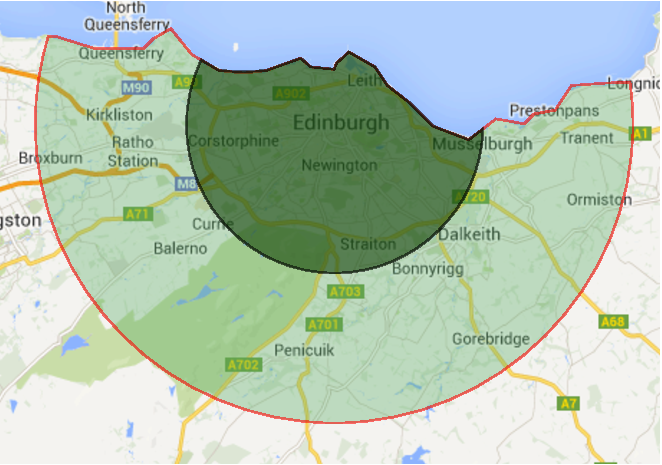
\includegraphics[width=0.9\textwidth]{edinburghmap}
      \caption[A map of Edinburgh]{A map of Edinburgh, with 5 and 10 mile radius ares displayed. A 5 mile radius circle includes the majority of the urban areas of Edinburgh city. Base image courtesy of Google Maps.}
      \label{edimap}
    \end{figure}
    Almost $4/5$ of missing people are found within the first 16 hours.
    According to information released from a survey of young runaways \cite{stillrunning}, 34\% of said they had been harmed or in a risky experience more than once,  and 11\% expressly said they had been hurt or harmed.
    It is critical to find at risk individuals, before they are harmed.
    Computer vision is already used to facilitate searches, but the volume of data available can exceed the capabilities of existing programs. %% cite cite cites 
    Furthermore, surveillance data from CCTV equipment produces data at real time speeds, so faster than real time processing speeds are desired.
    Real time speeds means that the program is able to analyse the data faster than it is being produced.
    This may involve reducing the amount of data being input i.e analysing 1 in every 30 images.
    Implementing a parallelised version of image recognition tools should greatly reduce the time an image takes to search.
    Governmental agencies, such as the police, could have access to very large computer systems, allowing for a high degree of parallelism.

    Another potential use can be found with surveying populations of wild animals.
    Wildlife conservation is a delicate task, which could benefit from rapid computer vision techniques.
    To accurately know which species are endangered, it is important to have an accurate count of the members of the species for a given region.
    Actively surveying the population by means of physically interacting with members can have adverse effects on the population.
    Nielsen \cite{electrofishing} discusses the negative effects of electrofishing on rare fish populations.
    She dicusses the lack of non-invasive methods of surveying the population, without which population counts cannot be maintained.
    Directly surveying endangered species can be inefficient, slow or dangerous to either the researcher or the animal in question.
    Passive techniques, such as photography, allow the researcher to estimate populations without interacting with the environment.
    Ideally a researcher would be constantly vigilant and able be to immediately identify each species correctly.
    This is rarely the case; a single human is fallible and a team is often beyond the funding of the endeavour.
    Instead, with access to any modern laptop and a digital camera, parallel computer vision may be able to assist in many ways.
    A video feed would allow observation for as long as the battery lasts, and a database of the features of regional species would help with identification.
    Parallel species recognition would allow multiple species to be surveyed at a time.
    It would allow non-experts to monitor the survey of the populations, freeing up experts for more specialised tasks.
      
    An everyday use of parallel object recognition is with nationwide traffic monitoring.
    Using existing roadside cameras, such as CCTV or speed cameras, a network could be built that monitors traffic on a large scale.
    This would help to improve commute times and general congestion issues, by advising drivers of congested areas and providing alternate routes.
    Paralleism could be applied to this situation.
    The sheer quantity of data for a large scale system like this would prevent real time analysis for a linear program.

    A simple and approachable usage case can be found in Where's Wally? puzzles.
    \subsection{Where's Wally? as a Test Case}
    %% Where's Wally? is a good basis for parallel object recognition
    %%    - maybe add a bit about clearly definable features?
    Where's Wally? puzzles are a good testbed for parallel computer vision.
    Each puzzle is a simple cartoon, a large image filled with various characters, who wear simply coloured clothing, see Figure \ref{justachump}.
    One of these characters is the eponymous Wally, who dresses distinctly from most others characters, see Figure \ref{justwally}.
    Similarly dressed characters exist, Figure \ref{justwenda}, to add complexity in finding Wally correctly.
    The cartoon nature of the characters means that shapes are boldly coloured and often bordered by a black line.
    As Where's Wally? is a puzzle, Wally will be hard to find; he can be obscured, camouflaged or simply small.
    Creating a program to solve Where's Wally? is non-trivial, requiring a combination of computer vision techniques.
    Thus the puzzle provides a good base to develop parallel object recognition.

    \begin{figure}[H]
    \centering
      \begin{subfigure}[b]{0.3\textwidth}
        \centering
        
\includegraphics[height=0.15\textheight]{just_a_chump}   
        \caption{A normal person}
        \label{justachump}
      \end{subfigure}
      \begin{subfigure}[b]{0.3\textwidth}
        \centering
        
\includegraphics[height=0.15\textheight]{just_wally}   
        \caption{Wally}
        \label{justwally}
      \end{subfigure}
      \begin{subfigure}[b]{0.3\textwidth}
        \centering
        
\includegraphics[height=0.15\textheight]{just_wenda}   
        \caption{Wenda}
        \label{justwenda}
      \end{subfigure}
    \caption{Characters from Where's Wally?}
    \label{wallychars}
    \end{figure}
    \subsection{Goals}
    This report presents Where's Wally? as a testbed to determine if High Performance Computer Vision can feasible used in in everyday life.
    This includes the production of a suite of functions that, though tuned to locating Wally, could be used to find other characters.
    The use of directive based parallelism will be added, to determine if a user-friendly system is viable.
    A simple and usable system is critical for everyday use.
    The more expertise required to implement parallel computer vision techniques, the fewer people are capable of creating solutions.
    Fewer solutions means that the problems will be restricted to the most practical problems, which in turn reduces the number of everyday applications.
    The generality of the suite of functions will be tested on non-Wally puzzles, to determine how generic the solution is.
    \subsection{Overview of Report}
    This report will begin by discussing the underlying information required to comprehend parallel object recognition.
    This includes literature reviews.
    The next section discusses the patterns used to recognise Wally.
    Each includes an analysis of the algorithm selection and a details of the level of parallelism which can be exposed.
    This will be used to produce a Where's Wally? solver, which examines the parallelism used to increase the speed of the Where's Wally solver.
    
    The report will comment on the results produced by the patterns and the solver.
    Following this, will be the concluding statements and ideas, along with recommendations for future use.
    The report will close with an evaluation of the project as a whole.
    Differences between the preparation phase and the actual report period will be noted here.
    \biblio
\end{document}
